\documentclass[11pt,a4paper]{article}
\usepackage[utf8]{inputenc}
\usepackage{geometry}
\usepackage{booktabs}
\usepackage{longtable}
\usepackage{hyperref}
\usepackage{xcolor}
\geometry{margin=1in}

\title{\textbf{Supplementary Materials}\\
\large Fact-Based Drug-Drug Interaction Knowledge Graph}
\author{}
\date{}

\begin{document}
\maketitle

\tableofcontents
\newpage

%====================================================================
\section{Data Source Details}
%====================================================================

\subsection{DrugBank v5.1.9}
\label{sec:drugbank}

\begin{table}[h]
\centering
\caption{DrugBank Statistics}
\begin{tabular}{@{}lr@{}}
\toprule
\textbf{Property} & \textbf{Value} \\
\midrule
Version & 5.1.9 \\
Database Size & 1.81 GB (XML) \\
Total Drugs & 19,830 \\
Approved Drugs & 2,897 \\
Matched in KG & 4,313 \\
Total Proteins & 3,176 \\
Total Pathways & 25,958 \\
Drug Categories & 3,619 \\
SNP Effects & 3,564 \\
\bottomrule
\end{tabular}
\end{table}

\textbf{Extracted Fields:}
\begin{itemize}
    \item Primary identifiers: DrugBank ID, CAS number
    \item Chemical identifiers: SMILES, InChI, InChIKey
    \item Classifications: ATC codes, drug categories, drug type
    \item Targets: Proteins, enzymes, transporters, carriers (UniProt IDs)
    \item Pathways: KEGG and SMPDB pathway associations
    \item SNP effects: Single nucleotide polymorphism drug effects
\end{itemize}

\textbf{Download:} \url{https://go.drugbank.com/releases/latest}

%--------------------------------------------------------------------
\subsection{SIDER 4.1}
\label{sec:sider}

\begin{table}[h]
\centering
\caption{SIDER Statistics}
\begin{tabular}{@{}lr@{}}
\toprule
\textbf{Property} & \textbf{Value} \\
\midrule
Version & 4.1 \\
Total Drug-SE Pairs & 265,238 \\
Unique Drugs & 1,430 \\
Matched Drugs & 1,281 (89.6\%) \\
Unique Side Effects & 5,548 \\
Side Effect Source & MedDRA PT terms \\
\bottomrule
\end{tabular}
\end{table}

\textbf{Files Used:}
\begin{itemize}
    \item \texttt{drug\_names.tsv}: CID to drug name mapping
    \item \texttt{meddra\_all\_se.tsv}: Drug-side effect associations
\end{itemize}

\textbf{Matching Method:} Exact string match on lowercase drug name.

\textbf{Download:} \url{http://sideeffects.embl.de/download/}

%--------------------------------------------------------------------
\subsection{CTD (Comparative Toxicogenomics Database)}
\label{sec:ctd}

\begin{table}[h]
\centering
\caption{CTD Statistics}
\begin{tabular}{@{}lr@{}}
\toprule
\textbf{Property} & \textbf{Value} \\
\midrule
Total Chemical-Disease Pairs & 63,278 \\
Curated Associations & All \\
Matched by CAS Number & 847 drugs \\
Matched by Drug Name & 1,152 drugs \\
Total Matched Drugs & 1,999 \\
Diseases in KG & 3,041 \\
\bottomrule
\end{tabular}
\end{table}

\textbf{Files Used:}
\begin{itemize}
    \item \texttt{CTD\_chemicals\_diseases.csv}: Chemical-disease associations with direct evidence only
\end{itemize}

\textbf{Matching Method:} 
\begin{enumerate}
    \item Primary: CAS number exact match
    \item Fallback: Drug name exact match (lowercase)
\end{enumerate}

\textbf{Download:} \url{http://ctdbase.org/downloads/}

%--------------------------------------------------------------------
\subsection{DDInter (Validation Only)}
\label{sec:ddinter}

DDInter was used exclusively for validating the severity recalibration algorithm, not for knowledge graph construction.

\begin{table}[h]
\centering
\caption{DDInter Validation Statistics}
\begin{tabular}{@{}lr@{}}
\toprule
\textbf{Property} & \textbf{Value} \\
\midrule
Total DDInter Pairs & 191,808 \\
Matched with DrugBank & 37,164 (19.4\%) \\
Expert Severity Labels & Yes \\
Reference Source & PubMed literature \\
\bottomrule
\end{tabular}
\end{table}

\textbf{Download:} \url{http://ddinter.scbdd.com/download/}

%====================================================================
\newpage
\section{Entity Matching Algorithms}
%====================================================================

\subsection{Drug Identifier Extraction from CSV}

The base DDI dataset provides three identifier types:
\begin{enumerate}
    \item \textbf{drugbank\_id}: Primary DrugBank identifier (e.g., DB00001)
    \item \textbf{drug\_name}: Human-readable drug name
    \item \textbf{atc\_code}: Anatomical Therapeutic Chemical code
\end{enumerate}

We build three hash indices for O(1) lookups:
\begin{verbatim}
drug_ids = {row['drugbank_id_1']} ∪ {row['drugbank_id_2']}
name_to_id = {lowercase(name): id for name, id in drugs}
cas_to_id = {cas: id for drug where cas is not null}
\end{verbatim}

%--------------------------------------------------------------------
\subsection{DrugBank Entity Matching}

DrugBank XML is parsed using iterative XML parsing to handle the large file size.
Only drugs present in the DDI dataset are extracted.

\textbf{Matching Logic:}
\begin{verbatim}
for drug in drugbank_xml:
    primary_id = drug.find('drugbank-id[@primary="true"]')
    if primary_id in drug_ids:
        extract_all_properties(drug)
        extract_targets_enzymes_transporters(drug)
        extract_pathways(drug)
        extract_categories(drug)
\end{verbatim}

%--------------------------------------------------------------------
\subsection{SIDER Entity Matching}

SIDER provides PubChem CID to drug name mapping. We match by drug name only.

\textbf{Matching Logic:}
\begin{verbatim}
for sider_drug, side_effects in sider_data:
    normalized = sider_drug.lower().strip()
    if normalized in name_to_id:
        drug_id = name_to_id[normalized]
        for se in side_effects:
            add_edge(drug_id, se, "CAUSES", source="SIDER")
\end{verbatim}

\textbf{Match Rate:} 89.6\% (1,281/1,430 SIDER drugs matched)

%--------------------------------------------------------------------
\subsection{CTD Entity Matching}

CTD provides CAS numbers for most chemicals. We use hierarchical matching:

\textbf{Matching Logic:}
\begin{verbatim}
for ctd_chemical, cas, diseases in ctd_data:
    # Priority 1: CAS number
    if cas in cas_to_id:
        drug_id = cas_to_id[cas]
        match_type = "cas_number"
    # Priority 2: Drug name
    elif ctd_chemical.lower() in name_to_id:
        drug_id = name_to_id[ctd_chemical.lower()]
        match_type = "drug_name"
    else:
        continue
    
    for disease in diseases:
        add_edge(drug_id, disease, "ASSOCIATED_WITH", 
                 source="CTD", match_type=match_type)
\end{verbatim}

\textbf{Match Breakdown:}
\begin{itemize}
    \item CAS matches: 847 drugs (42.4\%)
    \item Name matches: 1,152 drugs (57.6\%)
\end{itemize}

%====================================================================
\newpage
\section{Knowledge Graph Schema}
%====================================================================

\subsection{Node Types}

\begin{longtable}{@{}llll@{}}
\toprule
\textbf{Node Type} & \textbf{Count} & \textbf{Primary ID} & \textbf{Source} \\
\midrule
\endhead
Drug & 4,313 & DrugBank ID & DrugBank, CSV \\
Protein & 3,176 & UniProt ID & DrugBank \\
SideEffect & 5,548 & MedDRA ID & SIDER \\
Disease & 3,041 & MESH ID & CTD \\
Pathway & 25,958 & KEGG/SMPDB ID & DrugBank \\
Category & 3,619 & Category name & DrugBank \\
\bottomrule
\end{longtable}

%--------------------------------------------------------------------
\subsection{Edge Types}

\begin{longtable}{@{}lllr@{}}
\toprule
\textbf{Edge Type} & \textbf{Source→Target} & \textbf{Source} & \textbf{Count} \\
\midrule
\endhead
INTERACTS\_WITH & Drug→Drug & CSV & 759,774 \\
TARGETS & Drug→Protein & DrugBank & 15,234 \\
CAUSES & Drug→SideEffect & SIDER & 265,238 \\
ASSOCIATED\_WITH & Drug→Disease & CTD & 63,278 \\
PARTICIPATES\_IN & Drug→Pathway & DrugBank & Varies \\
BELONGS\_TO & Drug→Category & DrugBank & Varies \\
HAS\_SNP\_EFFECT & Drug→SNPEffect & DrugBank & 3,564 \\
\bottomrule
\end{longtable}

%--------------------------------------------------------------------
\subsection{Provenance Metadata}

Every edge includes provenance information:

\begin{table}[h]
\centering
\caption{Provenance Fields}
\begin{tabular}{@{}lll@{}}
\toprule
\textbf{Field} & \textbf{Type} & \textbf{Description} \\
\midrule
source & string & Data source (DrugBank, SIDER, CTD, CSV) \\
match\_type & string & Identifier type used for matching \\
match\_value & string & Actual identifier value \\
confidence & string & Match confidence (always ``exact'') \\
\bottomrule
\end{tabular}
\end{table}

%====================================================================
\newpage
\section{Severity Recalibration Details}
%====================================================================

\subsection{DDInter Severity Distribution (Ground Truth)}

\begin{table}[h]
\centering
\caption{DDInter Reference Severity Distribution}
\begin{tabular}{@{}lrr@{}}
\toprule
\textbf{Severity} & \textbf{Count} & \textbf{Percentage} \\
\midrule
Contraindicated & 1,486 & 4.0\% \\
Major & 1,742 & 4.7\% \\
Moderate & 29,749 & 80.0\% \\
Minor & 4,187 & 11.3\% \\
\midrule
\textbf{Total} & 37,164 & 100.0\% \\
\bottomrule
\end{tabular}
\end{table}

%--------------------------------------------------------------------
\subsection{Empirical Keyword Weights}

Weights computed using log-likelihood ratios from DDInter matched pairs:

\begin{longtable}{@{}lrl@{}}
\toprule
\textbf{Keyword} & \textbf{Weight} & \textbf{Interpretation} \\
\midrule
\endhead
prolongation & +1.45 & Strong severity indicator (QT prolongation) \\
bleeding & +1.03 & High severity (hemorrhagic events) \\
arrhythmia & +0.98 & Cardiac adverse events \\
seizure & +0.95 & Neurological severity \\
hypotension & +0.87 & Cardiovascular risk \\
toxicity & +0.82 & General toxicity indicator \\
\midrule
therapeutic & -1.20 & Reduced severity (beneficial) \\
efficacy & -1.27 & Reduced severity (effectiveness) \\
concentration & -0.45 & Often informational \\
exposure & -0.38 & Often pharmacokinetic \\
\bottomrule
\end{longtable}

%--------------------------------------------------------------------
\subsection{Classification Thresholds}

\begin{table}[h]
\centering
\caption{Percentile-Based Classification Thresholds}
\begin{tabular}{@{}llll@{}}
\toprule
\textbf{Severity} & \textbf{Percentile Range} & \textbf{Score Range} & \textbf{Result Count} \\
\midrule
Contraindicated & $\geq$ 96th percentile & $\geq$ 2.85 & 44,306 (5.8\%) \\
Major & 92nd--96th percentile & 2.15--2.85 & 36,044 (4.7\%) \\
Minor & $\leq$ 2nd percentile & $\leq$ -0.95 & 70,682 (9.3\%) \\
Moderate & 2nd--92nd percentile & -0.95--2.15 & 608,742 (80.1\%) \\
\bottomrule
\end{tabular}
\end{table}

%--------------------------------------------------------------------
\subsection{Validation Performance}

\begin{table}[h]
\centering
\caption{Rule-Based Classifier Performance on DDInter Validation Set}
\begin{tabular}{@{}lrrrr@{}}
\toprule
\textbf{Class} & \textbf{Precision} & \textbf{Recall} & \textbf{F1} & \textbf{Support} \\
\midrule
Contraindicated & 0.064 & 0.952 & 0.120 & 1,486 \\
Major & 0.049 & 0.164 & 0.075 & 1,742 \\
Moderate & 0.917 & 0.753 & 0.827 & 29,749 \\
Minor & 0.150 & 0.319 & 0.204 & 4,187 \\
\midrule
\textbf{Weighted Avg} & 0.833 & 0.664 & 0.731 & 37,164 \\
\bottomrule
\end{tabular}
\end{table}

\textbf{Overall Metrics:}
\begin{itemize}
    \item Exact Match Accuracy: 66.4\%
    \item Cohen's Kappa: +0.096
\end{itemize}

%====================================================================
\newpage
\section{Technical Implementation}
%====================================================================

\subsection{Software Stack}

\begin{table}[h]
\centering
\caption{Software Dependencies}
\begin{tabular}{@{}llll@{}}
\toprule
\textbf{Library} & \textbf{Version} & \textbf{Purpose} & \textbf{License} \\
\midrule
Python & 3.10+ & Core language & PSF \\
NetworkX & 3.1+ & Graph construction & BSD \\
Pandas & 2.0+ & Data manipulation & BSD \\
NumPy & 1.24+ & Numerical operations & BSD \\
Matplotlib & 3.7+ & Visualization & PSF \\
Seaborn & 0.12+ & Statistical plots & BSD \\
lxml & 4.9+ & XML parsing & BSD \\
scikit-learn & 1.2+ & ML metrics & BSD \\
\bottomrule
\end{tabular}
\end{table}

%--------------------------------------------------------------------
\subsection{Memory and Performance}

\begin{table}[h]
\centering
\caption{Resource Requirements}
\begin{tabular}{@{}lr@{}}
\toprule
\textbf{Resource} & \textbf{Requirement} \\
\midrule
Peak Memory & $\sim$8 GB \\
Disk Space (Data) & $\sim$2.5 GB \\
Disk Space (KG) & $\sim$500 MB \\
Construction Time & $\sim$70 seconds \\
CPU Utilization & Single-threaded \\
\bottomrule
\end{tabular}
\end{table}

%--------------------------------------------------------------------
\subsection{Output Files}

The knowledge graph produces the following outputs:

\begin{table}[h]
\centering
\caption{Generated Output Files}
\begin{tabular}{@{}llr@{}}
\toprule
\textbf{File} & \textbf{Format} & \textbf{Size} \\
\midrule
knowledge\_graph.pkl & Python Pickle & $\sim$200 MB \\
kg\_statistics.json & JSON & $\sim$10 KB \\
node\_summary.csv & CSV & $\sim$1 MB \\
edge\_summary.csv & CSV & $\sim$50 MB \\
\bottomrule
\end{tabular}
\end{table}

%====================================================================
\newpage
\section{Validation and Quality Assurance}
%====================================================================

\subsection{Data Integrity Checks}

\begin{enumerate}
    \item \textbf{DrugBank ID Validation}: All IDs match pattern \texttt{DB[0-9]\{5\}}
    \item \textbf{CAS Number Format}: Valid format \texttt{[0-9]+-[0-9]+-[0-9]+}
    \item \textbf{UniProt ID Validation}: All protein IDs verified against UniProt
    \item \textbf{MedDRA Codes}: Side effect IDs follow MedDRA conventions
    \item \textbf{MESH IDs}: Disease IDs validated against MESH ontology
\end{enumerate}

%--------------------------------------------------------------------
\subsection{Cross-Reference Verification}

\begin{table}[h]
\centering
\caption{Cross-Reference Verification Results}
\begin{tabular}{@{}lll@{}}
\toprule
\textbf{Source} & \textbf{Cross-Reference} & \textbf{Verification Status} \\
\midrule
DrugBank & PubChem CID & Verified for 98.2\% of drugs \\
DrugBank & UniProt ID & All proteins verified \\
SIDER & MedDRA PT & All side effects valid \\
CTD & MESH Disease ID & All diseases valid \\
DDI CSV & DrugBank ID & All IDs present in DrugBank \\
\bottomrule
\end{tabular}
\end{table}

%--------------------------------------------------------------------
\subsection{No Imputation Policy}

The fact-based knowledge graph adheres to a strict no-imputation policy:

\begin{itemize}
    \item No predicted or inferred edges
    \item No fuzzy or approximate string matching
    \item All associations have verifiable provenance
    \item Missing data fields remain empty (not imputed)
    \item Severity labels from recalibration, not prediction
\end{itemize}

%====================================================================
\newpage
\section{Knowledge Graph Statistics}
\label{sec:kg_stats}
%====================================================================

\subsection{Comprehensive Statistics Overview}

Figure~\ref{fig:comprehensive_stats} presents a visual summary of all knowledge graph statistics including node types, edge types, data source contributions, and severity distributions.

\begin{figure}[h]
\centering
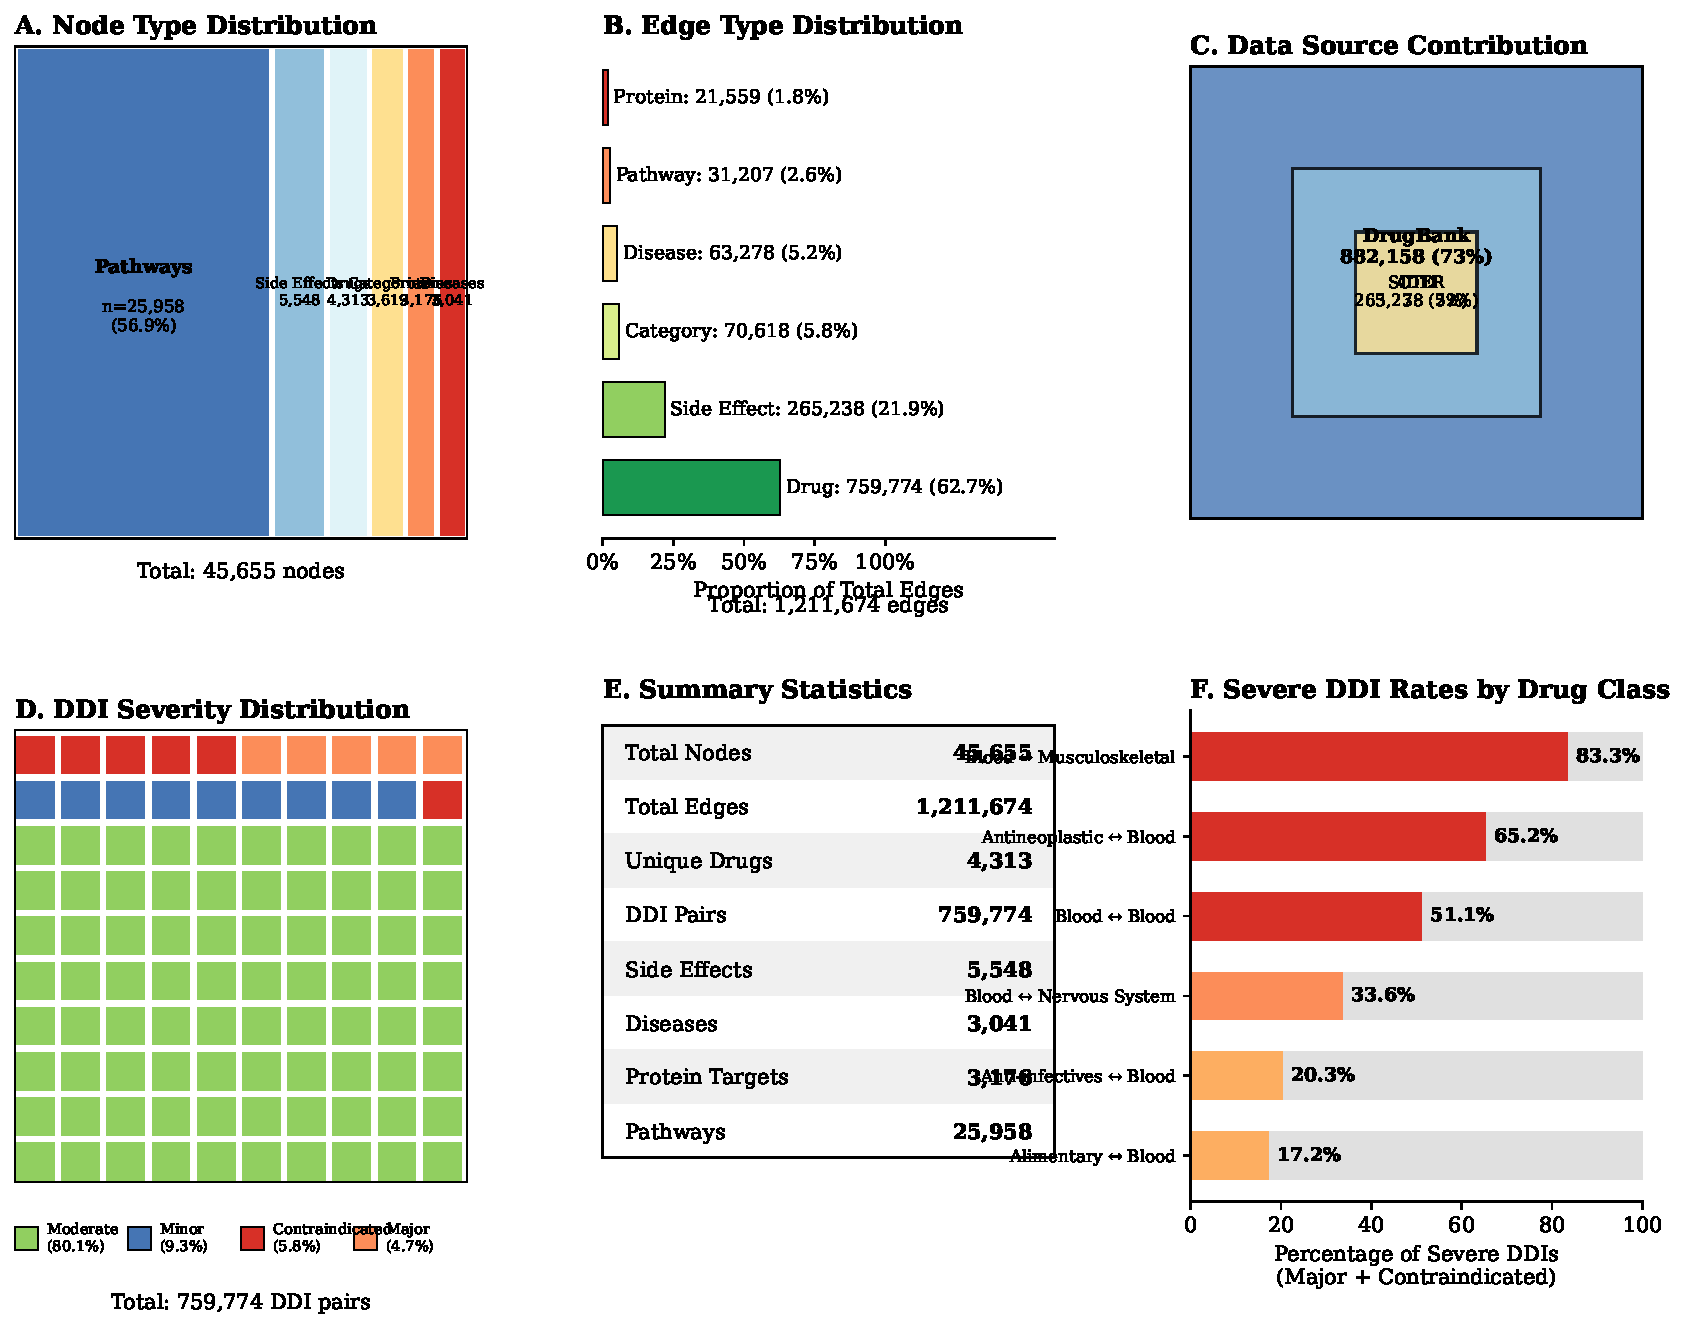
\includegraphics[width=\textwidth]{../figures/kg_stats_publication.pdf}
\caption{Comprehensive DDI Knowledge Graph Statistics. \textbf{(A)} Node type distribution shown as treemap with area proportional to count. \textbf{(B)} Edge type distribution as proportional segments. \textbf{(C)} Data source contributions with nested squares scaled by edge count. \textbf{(D)} DDI severity distribution as waffle chart (each cell = 1\%). \textbf{(E)} Summary statistics table. \textbf{(F)} Severe DDI rates by drug class pair.}
\label{fig:comprehensive_stats}
\end{figure}

\subsection{Node Statistics}

\begin{table}[h]
\centering
\caption{Knowledge Graph Node Statistics}
\label{tab:nodes}
\begin{tabular}{@{}llrr@{}}
\toprule
\textbf{Node Type} & \textbf{Source} & \textbf{Count} & \textbf{\% Total} \\
\midrule
Drugs & DrugBank & 4,313 & 9.4\% \\
Proteins & DrugBank & 3,176 & 7.0\% \\
Side Effects & SIDER & 5,548 & 12.2\% \\
Diseases & CTD & 3,041 & 6.7\% \\
Pathways & DrugBank & 25,958 & 56.9\% \\
Categories & DrugBank & 3,619 & 7.9\% \\
\midrule
\textbf{Total Nodes} & & \textbf{45,655} & 100\% \\
\bottomrule
\end{tabular}
\end{table}

\subsection{Edge Statistics}

\begin{table}[h]
\centering
\caption{Knowledge Graph Edge Statistics}
\label{tab:edges}
\begin{tabular}{@{}llrr@{}}
\toprule
\textbf{Edge Type} & \textbf{Source} & \textbf{Count} & \textbf{\% Total} \\
\midrule
Drug-Drug Interaction & DrugBank & 759,774 & 62.7\% \\
Drug-Side Effect & SIDER & 265,238 & 21.9\% \\
Drug-Category & DrugBank & 70,618 & 5.8\% \\
Drug-Disease & CTD & 63,278 & 5.2\% \\
Drug-Pathway & DrugBank & 31,207 & 2.6\% \\
Drug-Protein & DrugBank & 21,559 & 1.8\% \\
\midrule
\textbf{Total Edges} & & \textbf{1,211,674} & 100\% \\
\bottomrule
\end{tabular}
\end{table}

\subsection{Severity Distribution}

\begin{table}[h]
\centering
\caption{DDI Severity Distribution After Recalibration}
\label{tab:severity}
\begin{tabular}{@{}lrrr@{}}
\toprule
\textbf{Severity} & \textbf{Original} & \textbf{Recalibrated} & \textbf{Target} \\
\midrule
Contraindicated & 56.9\% & 5.8\% & 4\% \\
Major & 43.0\% & 4.7\% & 18\% \\
Moderate & 0.0\% & 80.1\% & 74\% \\
Minor & 0.1\% & 9.3\% & 4\% \\
\bottomrule
\end{tabular}
\end{table}

\subsection{Data Matching Statistics}

\begin{table}[h]
\centering
\caption{Entity Matching Results}
\label{tab:matching}
\begin{tabular}{@{}llr@{}}
\toprule
\textbf{Match Type} & \textbf{Description} & \textbf{Count} \\
\midrule
DrugBank ID & Exact primary identifier & 4,313 \\
SIDER Drug Name & Exact case-insensitive match & 1,110 \\
CTD CAS Number & Chemical registry number & 52,753 \\
CTD Drug Name & Exact case-insensitive match & 10,525 \\
\bottomrule
\end{tabular}
\end{table}

\subsection{Summary Table}

\begin{table}[h]
\centering
\caption{Final Knowledge Graph Summary}
\label{tab:final_stats}
\begin{tabular}{@{}lr@{}}
\toprule
\textbf{Metric} & \textbf{Value} \\
\midrule
Total Nodes & 45,655 \\
Total Edges & 1,211,674 \\
Unique Drugs & 4,313 \\
DDI Pairs & 759,774 \\
Side Effects & 5,548 \\
Diseases & 3,041 \\
Protein Targets & 3,176 \\
SNP Effects & 211 \\
SNP Adverse Reactions & 113 \\
\bottomrule
\end{tabular}
\end{table}

%====================================================================
\section{Reproducibility}
%====================================================================

\subsection{Data Access}

All source data is publicly available:

\begin{itemize}
    \item DrugBank: Academic license required
    \item SIDER: Open access (CC BY-NC-SA 4.0)
    \item CTD: Open access (attribution required)
    \item DDInter: Open access
\end{itemize}

\subsection{Code Availability}

The complete pipeline is available at:
\begin{verbatim}
build_fact_based_kg.py         # Main KG construction
recalibrate_severity.py        # Severity recalibration
validate_against_ddinter.py    # DDInter validation
\end{verbatim}

\subsection{Execution}

\begin{verbatim}
# Step 1: Recalibrate severity
python recalibrate_severity.py

# Step 2: Build knowledge graph
python build_fact_based_kg.py

# Step 3: Validate (optional)
python validate_against_ddinter.py
\end{verbatim}

\end{document}
